\section[The three limit regimes]{The three limit regimes and their dimensionless description}

\label{2302:sec:regimes}
As discussed before, the optimization problem introduced in Sec.~\ref{2302:sec:setting} defines a non-convex optimization problem. Moreover, modern neural networks operate in a regime where both the data dimension $d$ and the number of parameters in the network $\hids$ are large. Therefore, characterizing the evolution of the weights $\Theta^{\i}\in\mathbb{R}^{\hids(d+1)}$ amounts to studying $\hids(d+1)$ non-linear, coupled, non-convex stochastic process - a challenging problem even for numerical methods. As motivated in the introduction Sec.~\ref{2302:sec:intro}, in this section we derive a \emph{tractable}, \emph{low-dimensional} description for SGD in different regimes of practical interest. 

\subsection{Main concepts}

\paragraph{Sufficient statistics:} A first observation is that the performance of the predictor $(\Theta^{\i})_{\i\leq \nsamp}$ at iteration $\i \leq n$ only depends on the statistics of the student and teacher pre-activations 
\begin{equation}\label{2302:eq:def:pre_activations}
    \vec{\lambda}^{\i}\coloneqq \mat{W}^{\i}\vec{x}^{\i}\in\mathbb{R}^{\hids}, \quad {\vec{\lambda}^{\star}}^{\nu}\coloneqq\mat{W}^{\star}\vec{x}^{\i}\in\mathbb{R}^{\hidt}
\end{equation}
Moreover, since $\vec{x}^\i$ is Gaussian and independent of $(\mat{W}^{\i}, \mat{W}^{\star})$, the pre-activations are jointly Gaussian vectors $(\vec{\lambda}^{\i}, {\vec{\lambda}^{\star}}^{\nu})\sim\mathcal{N}(\vec{0}_{\hids+\hidt}, \Omega^{\i})$ with covariance: 
\begin{equation}\label{2302:eq:def:overlaps}
\begin{split}
\Omega^{\i}\coloneqq
\begin{pmatrix}
\mat{Q}^{\i}& \mat{M}^{\i}\\
{\mat{M}^{\i\top}} & \P
\end{pmatrix}=
\begin{pmatrix}
\sfrac{1}{d}\mat{W}^{\i}{\mat{W}^{\i}}^{\top}& \sfrac{1}{d}\mat{W}^{\i}{\mat{W}^{\star}}^{\top}\\
\sfrac{1}{d}\mat{W}^{\star}{\mat{W}^{\i}}^{\top}& \sfrac{1}{d}\mat{W}^{\star}{\mat{W}^{\star}}^{\top}
\end{pmatrix}
\in\mathbb{R}^{(\hids+\hidt)\times (\hids+\hidt)}
\end{split}
\end{equation}
which is the \emph{sufficient statistics} matrix for the population risk in Equation~\eqref{2302:eq:def:poprisk}. Massaging Equation~\eqref{2302:eq:def:sgd}, we can derive a closed set of stochastic processes governing the evolution of the sufficient statistics:
\begin{equation}
\label{2302:eq:def:overlap_process}
\begin{split}
M^{\i+1}_{ir} - M^{\i}_{ir} &= \frac{\gamma}{\hids d}\sigma'(\lambda_i^\i)\lambda^{\star\i}_{r}  \mathcal{E}^{\i}\\
Q_{ij}^{\i+1} - Q^{\i}_{ij} &=  \frac{\gamma}{\hids d}\left(\sigma'(\lambda_i^\i)\lambda^{\i}_{j}+\sigma'(\lambda_j^\i)\lambda^{\i}_{i}\right) \mathcal{E}^\i+\frac{\gamma^2 ~||\vec{x}^{\i}||_{2}^{2}}{p^2d}	\sigma'(\lambda_i^\i)\sigma'(\lambda_j^\i) {\mathcal{E}^{\i}}^2
\end{split}
\end{equation}
where we defined for convenience the displacement vector 
\begin{equation}
\mathcal{E}^{\i} \coloneqq \frac{1}{k}\sum_{r=1}^{\hidt}\sigma^{\star}(\lambda_{r}^{\star\i})-\frac{1}{p}\sum_{j=1}^{\hids}\sigma(\lambda_{j}^{\nu})+\sqrt{\noise} z^{\i}.
\end{equation}
Note that so far we have made no approximations: these equations are exact, and allow us to trade the $\hids(d+1)$ dimensional process for $\Theta^{\i}$ in Equation~\eqref{2302:eq:def:sgd} for a $\hids(\hidt+\hids)$ dimensional process for $(\mat{M}^{\i},\mat{Q}^{\i})$. This can be particularly convenient if $d\gg \hidt, \hids$. 

The process in Equation~\eqref{2302:eq:def:overlap_process} has been previously studied in different limits and particular cases. For instance, \cite{tan2019online} studied the stochastic dynamics in particular case of $\hidt=\hids=1$ and $\sigma(x)=x^2$, also known as \emph{phase retrieval}, and \cite{arous2021online} extended this discussion for arbitrary $\sigma$. More important to our work, \cite{saad1995line,saad1996dynamics} has shown that this process admits a deterministic limit when $d \to \infty$ at fixed $p,\gamma$, characterized by the following ODE:
\begin{align}
\label{2302:eq:def:ss_ode}
\frac{\dd \mat{M}}{dt} = \Psi^{(\mathrm{M})}(\Omega), &&
\frac{\dd\mat{Q}}{\dd t} =  \Psi^{(\mathrm{GF})}(\Omega) +\frac{\gamma}{p} \Psi^{(\mathrm{Var})}(\Omega),
\end{align}
where the right-hand side functions are defined by the following equations.
\begin{equation} \label{2302:eq:def:Psi}
\begin{split}
\Psi^{(\mathrm{M})}_{ir}(\Omega) &= \mathbb E_{(\vec{\lambda},\vec{\lambda}^{\star})\sim\mathcal{N}(\vec{0}_{\hids+\hidt}, \Omega)} \left[\sigma'(\lambda_i)\lambda^{\star}_{r} \mathcal{E}\right]\\
\Psi^{(\mathrm{GF})}_{ij}(\Omega) &=  \mathbb E_{(\vec{\lambda},\vec{\lambda}^{\star})\sim\mathcal{N}(\vec{0}_{\hids+\hidt}, \Omega)} \left[\left(\sigma'(\lambda_i)\lambda_{j}+\sigma'(\lambda_j)\lambda_{i}\right) \mathcal{E}\right] \\
\Psi^{(\mathrm{Var})}_{ij}(\Omega) &= \mathbb E_{(\vec{\lambda},\vec{\lambda}^{\star})\sim\mathcal{N}(\vec{0}_{\hids+\hidt}, \Omega)} \left[\sigma'(\lambda_i)\sigma'(\lambda_j) {\mathcal{E}}^2 \right]
\end{split}
\end{equation}
As will be discussed later in Section \ref{2302:sec:classic}, the superscript notation for the right-hand side is suggestive of their interpretation. This convergence was made rigorous by \cite{goldt2019dynamics} and \cite{veiga2022phase}, who showed the following non-asymptotic result:

\begin{theorem} [\cite{veiga2022phase}] \label{2302:th:conv_eps} We place ourselves under Assumptions \ref{2302:assump:boundedness}-\ref{2302:assump:activation}. Let $\Omega^\i$ be the random process of Equation~\eqref{2302:eq:def:overlap_process}, and $\Omega(t)$ the solution to the ODE \eqref{2302:eq:def:ss_ode} with starting point $\Omega(0) = \Omega^0$. Define the step-size $\delta t = \sfrac{\gamma}{pd}$, and assume that $\gamma / p = O(1)$.
Then there exists a constant $C > 0$ such that for any $\i \geq 0$,
\begin{equation}
    \lVert \Omega^{\nu} - \Omega(\nu\delta t) \rVert_\infty \leq e^{C\i \delta t} \sqrt{\frac{\gamma}{pd}}
\end{equation}
\end{theorem}

\cite{veiga2022phase} also described the behavior of $\Omega$ for various choices of $\gamma$ and $p$. In particular, when $\gamma / p \ll 1$, equations \eqref{2302:eq:def:ss_ode} reduce to the following simpler ones:
\begin{align}
\label{2302:eq:def:gf_ode}
\frac{\dd\mat{M}}{\dd t} = \Psi^{(\mathrm{M})}(\Omega), && 
\frac{\dd\mat{Q}}{\dd t} =  \Psi^{(\mathrm{GF})}(\Omega)
\end{align}
Our key observation is that the deterministic description above is valid beyond the high-dimensional limit $d\to\infty$ on which previous works \citep{saad1995line,goldt2019dynamics,veiga2022phase} have focused. Indeed, Theorem~\ref{2302:th:conv_eps} is non-asymptotic in $(d,\hids,\gamma)$, and can thus be applied in any setting where $\sfrac{\gamma}{pd} \ll 1$. This is leveraged to provide a tractable, low-dimensional description of SGD in different scenarios of interest which we summarize in Fig.~\ref{2302:fig:triangle}. 

%%%%%%%%%%%%%%%%%%%%%%%%%%%%%%%%%%%%%%%%%%%%
\subsection{The classical regime}
\label{2302:sec:classic}
%%%%%%%%%%%%%%%%%%%%%%%%%%%%%%%%%%%%%%%%%%%%
The first and most well-studied scenario is the classical regime in which $\gamma\to 0^{+}$ at fixed dimensions $d, \hids = O(1)$.  Defining the continuous weight $\Theta^{\i} = \Theta(\nu\delta t)$ via linear interpolation, a classical result from stochastic optimization  \citep{robbins1951stochastic} is that one-pass SGD converges to gradient flow on the population risk:
\begin{align}
\label{2302:eq:gf}
\frac{\dd \Theta(t)}{\dd t} = -\nabla_{\Theta}\mathcal{R}(\Theta(t)) 
\end{align}
Or in words: the effective SGD noise $\varepsilon_{\nu}$ in Equation~\eqref{2302:eq:sgd:noise} is subleading in this limit. Note that this is a deterministic ordinary differential equation of dimension $\hids(d+1)$. Since $d,\hids = O(1)$, if they are small Equation~\eqref{2302:eq:gf} provides a computationally efficient description of the SGD dynamics, since it can be easily implemented and solved in a computer. Nonetheless, an alternative description can be derived from the sufficient statistics of Equation~\eqref{2302:eq:def:overlaps}. Indeed, Theorem~\ref{2302:th:conv_eps} guarantees that in the limit $\gamma\to 0^{+}$, the stochastic process in Equation~\eqref{2302:eq:def:overlap_process} converges to the deterministic limit of Equation~\eqref{2302:eq:def:gf_ode}. This ODE can be easily seen to be equivalent to the one of \eqref{2302:eq:gf}, through the following identity:
\[ \frac{\dd  \langle \vec{w_i}, \vec{w_j} \rangle}{\dd{t}} = \left\langle \vec{w_i}, \frac{\dd\vec{w_j}}{\dd{t}} \right\rangle + \left\langle \frac{\dd\vec{w_i}}{\dd{t}}, \vec{w_j} \right\rangle \]
This gives rise to ordinary differential equations in $\hids (\hidt+\hids)$ parameters. Therefore, depending on the values of $(d,\hids)$, it can offer a more compact description of the evolution of the performance of the predictor than Equation~\eqref{2302:eq:gf}. 

As it was previously hinted by the notation, equation \eqref{2302:eq:def:gf_ode} also provides an intuitive interpretation of the right-hand side of the stochastic process \eqref{2302:eq:def:overlap_process}. Indeed, the terms proportional to $\sfrac{\gamma}{\hids d}$ in Equation~\eqref{2302:eq:def:overlap_process} correspond exactly to the terms inside the expectation in Equation~\eqref{2302:eq:def:gf_ode}, and correspond to the projection of the population gradient along the weights $(\Theta, \Theta_{\star})$. The remaining term, which is proportional to $\sfrac{\gamma^2}{\hids^2 d}$, comes from the variance of the effective noise $\varepsilon$, which is subleading in the limit $\gamma\to 0^{+}$. This agrees with the characterization of the terms given in \cite{arous2022high}, where an additional Brownian motion correction term at finer scales is also derived.

In Figure~\ref{2302:fig:classic-limit}~(left) we plot the trajectories of individual neurons in the space spanned by the two target neurons (\(k=2\)); \(\sfrac{\M_{jr}}{\sqrt{\Q_{jj}\P_{rr}}}\) is the (normalized) scalar product between \(\w_j\) and \(\w^*_r\). While, initially, all neurons are moving towards the superposition of the two teacher weights (\((\sfrac{\sqrt2}{2},\sfrac{\sqrt2}{2})\), yellow dot), in the last phase of learning they ``specialize'' and split evenly to one of the two (\((1,0),(0,1)\), red squares). Note how the ODE trajectories follows closely the simulated ones, given the specific initialization.

Finally, our results imply a remarkable {\bf dimension independence} property: Differently from \eqref{2302:eq:gf}, the alternative description \eqref{2302:eq:def:gf_ode} turns out to be independent of the data dimension $d$. Given the initial conditions of the sufficient statistics (the overlaps), then the trajectories will behave {\bf exactly in the same way} whether $d$ is large or small (see the illustration in Figure~\ref{2302:fig:classic-limit}~(right)). This remarkable property is a direct consequence of the Gaussianity assumption on the data. Note, of course, that dimensionality still plays a crucial role through the initialization. Indeed, for the typically employed random initialization $\theta_{i}^{0}\sim\mathcal{N}(0_{d},\sigma^2\mat{I}_{d})$, the initial correlation between the hidden-units and the target, parameterized by $M^{0}_{rj}\sim \sfrac{1}{\sqrt{d}}$, explicitly depends on $d$. Since $M = 0$ is often a fixed-point of the dynamics, $d = O(1)$ or $d \gg 1$ will lead effectively to different behaviors. 

\begin{figure}
    \centering
        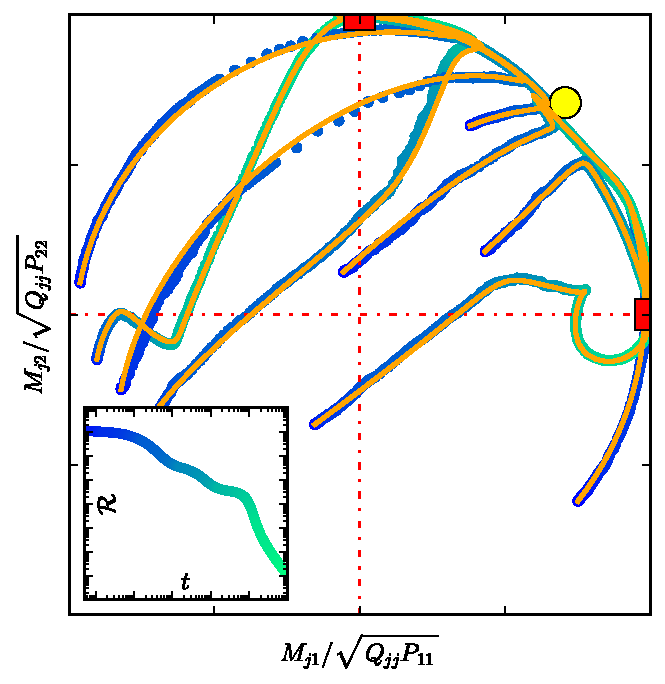
\includegraphics[width=0.44\textwidth]{figs/classic/classic_limit-particle-plot_gamma=0.05--id2-ic_id3}
        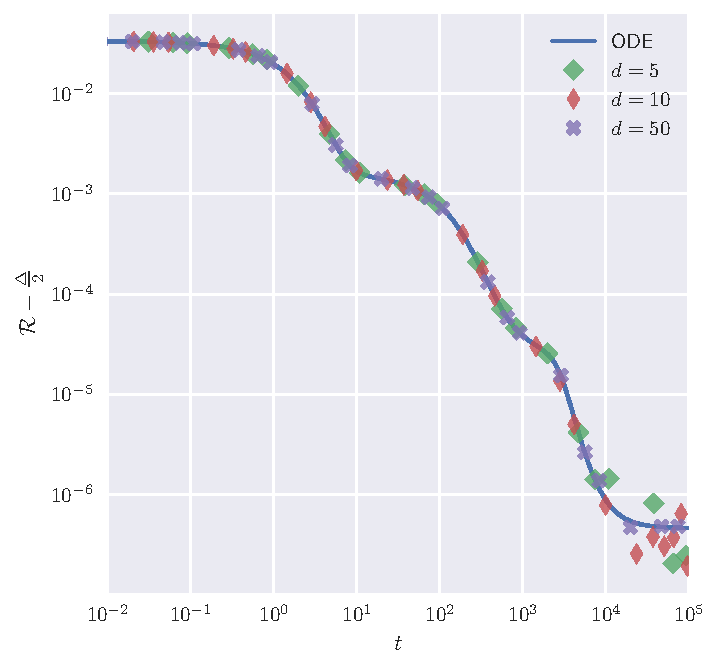
\includegraphics[width=0.49\textwidth]{figs/classic/classic_limit_d_plot_-k5_p10_noise0.001_gamma0.0500}
    \caption{{\bf Dimension independence of the dynamics in the classical regime}:
Comparison between the simulated SGD  dynamic and the analytical one obtained by integrating the differential equations. All the plots are using $\sigma=\erf(\sfrac{\cdot}{\sqrt{2}})$. (Left) Trajectories for the cosine similarity between each network neural and the target; time evolution in simulation is blue to green, ODE trajectories in orange (\(\hidt=2,\hids=10,\lr=\num{5e-2},\noise=\num{0.}\)). (Right)  Different low-dimensional simulations, starting from the same identical initial condition (\(\hidt=5,\hids=10,\lr=\num{5e-2},\noise=10^{-3}            \)).
    }
    \label{2302:fig:classic-limit}
\end{figure}

%%%%%%%%%%%%%%%%%%%%%%%%%%%%%%%%%%%%%%%%%%%%
\subsection{The high-dimensional regime}
\label{2302:sec:saadsolla}
%%%%%%%%%%%%%%%%%%%%%%%%%%%%%%%%%%%%%%%%%%%%
Modern machine learning practice often involves high-dimensional data. As early as in
\citep{saad1995line,saad1996dynamics} it has motivated the study of the $d\to\infty$ limit of the SGD dynamics \eqref{2302:eq:sgd:noise}, under the assumption of fixed learning rate and model complexity $p,\gamma = O(1)$. This setting has witnessed a renewal of interest recently \cite{vershynin2018high,goldt2019dynamics,veiga2022phase,arous2022high}. In particular, a remarkable phenomenon arises: differently from the classical limit Equation~\eqref{2302:eq:def:gf_ode} discussed above, in high-dimension the variance term induced by the SGD effective noise yields an explicit contribution to the limiting dynamics \eqref{2302:eq:def:ss_ode}. This term can yield a finite risk contribution at large times even for architectures for which the population gradient flow would otherwise converge to zero population risk  (i.e. perfect learning of the target $f_{\Theta^{\star}}$), so that the large time dynamics plateau at finite risk (see for instance \cite{goldt2019dynamics,arous2022high}). This is a major difference between the classical and high-dimensional regime.

For strongly convex problems, it is known that SGD with fixed learning rate $\gamma$ converges to a stationary distribution of variance $\propto \gamma$ \cite{pflug1986stochastic,dieuleveut2020bridging}, leading to an asymptotic risk that closely resembles the one observed by \cite{saad1995line} in the high-dimensional regime. This suggests a similar phenomenology in the basin of the global minima, although making this statement precise is challenging due to the non-convexity of the risk for two-layer networks.  As noted by \cite{veiga2022phase}, this noise term is subleading in $\sfrac{\gamma}{p}$, and can be mitigated by either taking $\gamma\to 0^{+}$ (i.e. seeing a lot of data) or overparametrizing $\hids\to\infty$. However, since eqs.~\eqref{2302:eq:def:ss_ode} are a system of $\hids(\hids+\hidt)$ ordinary differential equations, they become intractable in the limit $\hids\to\infty$, which is a major shortcoming of this description. 

%%%%%%%%%%%%%%%%%%%%%%%%%%%%%%%%%%%%%%%%%%%%
\subsection{The overparametrized regime}
\label{2302:sec:meanfield}
%%%%%%%%%%%%%%%%%%%%%%%%%%%%%%%%%%%%%%%%%%%%
In both the classical and high-dimensional regimes, the effective description of the SGD dynamics rely on quantities which scale with the hidden-layer width $\hids$, and therefore they are not adequate to wide models. Yet, in many scenarios of interest we need to deal with wide, overparametrized networks. The problem is finding an effective low-dimensional description of one-pass SGD for the overparametrized regime $\hids\to\infty$ was first addressed by \cite{mei2018mean,chizat2018global,rotskoff2022trainability,sirignano2020mean}. The key idea in this line of work is to define an empirical density over the weights $\theta^{\i}_{i}\coloneqq (a_{i}^{\i},\vec{w}^{\i}_{i})$:
\begin{align}
\hat{\mu}^{\i}_{\hids}(\vec{\theta}) = \frac{1}{p}\sum\limits_{i=1}^{\hids} \delta(\vec{\theta}-\vec{\theta}_{i}^{\i})
\end{align}
 and to derive a closed-form update for the density $\hat{\mu}^{\i}_{\hids}(\vec{\theta})$ from the SGD update of the weights, Equation~\eqref{2302:eq:sgd:noise}. In the limit $\hids\to\infty$, those works have shown that the empirical density converges to an asymptotic density over $\mathbb{R}^{d+1}$, which for sufficiently small learning rate satisfies a partial differential equation (PDE) that became known in the literature as the \emph{mean-field limit}. Drawing from the theory of PDEs and optimal transport, this description allowed for the derivation of important mathematical guarantees on the dynamics, such as the global convergence of SGD for two-layers neural networks. 

However, the empirical measure $\hat \mu_p^\nu$ is defined on $\mathbb R^{d+1}$, so a problem still remains when $d$ is large. Indeed, as remarked in \cite{bach2022gradient} it remains challenging to draw quantitative results from this description except for considerably low-dimensional data. However, since in our setting the target function \eqref{2302:eq:target} only acts on a low-dimensional subspace of $\mathbb R^d$, it is possible to exploit the symmetries of the problem to derive an approximation of constant dimension. This low-dimensional equivalent stems from invariance properties of mean-field equations, which were also used in \cite{abbe2022merged} and studied in depth in \cite{hajjar2023symmetries}. However,  \cite{abbe2022merged} only considers the $d \to \infty$ limit, while we derive a limit that is valid for any value of $d$.  \cite{hajjar2023symmetries}, on the other hand, is closer to our work (see e.g. their Lemma 4.2), but only handles the approximation of the dynamics by PDEs instead of ODEs.

\paragraph{Decomposing the dynamics:} The starting point of this low-dimensional description is the decomposition of $W$ as
\begin{equation}\label{2302:eq:W_proj}
    W = W_{\text{proj}} + W^\bot,
\end{equation}
where $W_{\text{proj}}$ is the orthogonal projection on the teacher vectors $W^\star$. This projection can be expressed using the sufficient statistics defined in Equation~\eqref{2302:eq:def:overlaps}:
\begin{equation}\label{2302:eq:W_proj_simplified}
    W =  M P^{-1} W^\star + W^\bot.
\end{equation}
Similar to \eqref{2302:eq:def:pre_activations}, we can then define the orthogonal pre-activations and its covariance matrix:
\begin{align}\label{2302:eq:def:lambda_orth}
    \vec{\lambda}^{\bot\i} &= W^{\bot\i}\vec{x}^\i \\
    \label{2302:eq:def:Qorth}
    Q^\bot &= \sfrac{1}{d} W^\bot (W^\bot)^\top = Q - MP^{-1}M^\top  .
\end{align}
Since we are in a regime where $\gamma / p \ll 1$, the ODE approximation of SGD corresponds to equations \eqref{2302:eq:def:gf_ode}. From there, with a little algebra (see Appendix \ref{2302:app:mean_field_orthogonal_derivation}), we can derive the corresponding equations for $Q^\bot$:
\begin{equation} \label{2302:eq:def:mf_orthogonal}
    \frac{dQ_{ij}^\bot}{dt} =  \mathbb E_{(\vec{\lambda}^{\bot},\vec{\lambda})}\left[\left( \sigma'(\lambda_i)\lambda_j^\bot + \sigma'(\lambda_j)\lambda_i^\bot \right) \mathcal{E} \right] \coloneqq \Psi^\bot_{ij}(\Omega).
\end{equation}

\paragraph{Low-dimensional approximation:} Informally, the interesting part of the dynamics happens in a low-dimensional space: the one spanned by the target weights $W^\star$. The remainder of the dynamics only depends on the student-student vector interactions, which are orthogonally invariant. We therefore make the following assumption to enforce this invariance at the start:
\begin{assump}\label{2302:assump:init}
    The initial vectors $(\vec{w}_1, \dots, \vec{w}_p)$ are drawn i.i.d from an orthogonally invariant and $\sfrac{K^2}{d}$-subgaussian distribution $\mu_0$, for some constant $K > 0$.
\end{assump}

We show in the appendix how we can then approximate the dynamics by only tracking the evolution of $M$ and $\mathrm{diag}(Q^\bot)$, and using the following ansatz:
\begin{equation}
\label{2302:eq:mf_approx_lowd}
    \vec{w}^\bot_i \approx \sqrt{q_{ii}^\bot} \cdot \vec{g}_i,
\end{equation}
where $\vec{g}_i$ are i.i.d uniform random variables on $\mathcal S^{d-k-1}$ independent from the $q_{ii}^\bot$. More precisely, we consider the reduced parameters $\tilde\Theta = (M, q) \in \mathbb R^{p(k+1)}$, and the following mean-field equivalent of the  overlaps:
\begin{equation}
\label{2302:eq:def:overlaps_mf}
\tilde\Omega = \begin{pmatrix} \tilde Q & M \\
    M^\top & P 
\end{pmatrix}, \quad \tilde{Q} = MP^{-1}M^\top +   D_{\sqrt{q}} \Xi D_{\sqrt{q}}
\end{equation}
where $D_{\sqrt{q}}$ is the diagonal matrix whose entries are the $\sqrt{q_{i}}$, and $\Xi$ is a \emph{random} matrix with independent entries such that
\[\Xi_{ii} = 1, \quad \Xi_{ij} = \langle \vec{g}, \vec{g'} \rangle \quad \text{with}\quad  \vec{g}, \vec{g'} \sim \mathrm{Unif}\left(\mathbb S^{d-k-1}\right)\]
Then, the mean-field ODEs read
\begin{equation}
\label{2302:eq:def:mf_ode}
    \frac{\dd M}{\dd t} = \mathbb{E}_{\Xi}\left[\Psi^{(M)}(\tilde\Omega)\right] \quad \frac{\dd q_i}{\dd t} = \mathbb{E}_{\Xi}\left[\Psi^{\bot}_{ii}(\tilde\Omega)\right].
\end{equation}
Similarly, given the parameters $\Theta$, the risk is computed as
\begin{equation}\label{2302:eq:def:mf_risk}
    \mathcal{R}(\tilde\Theta) = \mathbb{E}_{\Xi}\left[\mathcal{R}(\tilde\Omega)\right]
\end{equation}
The consistency of this approximation is given by the following theorem:
\begin{theorem}\label{2302:thm:mf_approx_lowd_bound}
 Under Assumptions~\ref{2302:assump:activation}~and~\ref{2302:assump:init}, let $\mat{\Omega}(t)$ and $\tilde{\mat{\Theta}}(t)$ denote the solutions of the ODES \eqref{2302:eq:def:gf_ode} and \eqref{2302:eq:def:mf_ode}, respectively. Then with probability at least $1 - e^{-z^2}$ on the initialization:
    \[ \sup_{t \in [0, T]} \left| \mathcal R(\mat{\Omega}(t)) - \mathcal R(\tilde{\mat{\Theta}}(t)) \right| \leq {Ce^{CT} \left(\sqrt{\log(pT)} + z \right)}/{\sqrt{p}} .\]
\end{theorem}
The proof is given in Appendix \ref{2302:sec:app:mf}. It uses key elements from the mean-field study of \cite{mei2019mean}. Indeed, both the solutions of \eqref{2302:eq:def:gf_ode} \& \eqref{2302:eq:def:mf_ode} can be viewed as the ``particle dynamics'' approximations (see e.g. \cite{chertock2017practical}) of two mean-field PDEs $\mu_t, \tilde\mu_t$ on the space of network weights $\vec{w} \in \mathbb{R}^{d}$ and the space or reduced parameters $(\vec{m}, q) \in \mathbb{R}^{k+1}$, respectively. In turn, the invariance property of $\mu_0$ extends to $\hat\mu_t$ for every $t \geq 0$, which implies that $\mathcal R(\mu_t) = \mathcal R(\tilde\mu_t)$. 

\begin{remark}
    We do not imply in any way, shape or form that Equation \eqref{2302:eq:mf_approx_lowd} represents the actual distribution of the $\vec{w}_i^\bot$, or that (as in \eqref{2302:eq:def:overlaps_mf}) then entries of $Q^\bot$ are independent. Rather, it is the structure of the update equations that allows for this approximation to hold.
\end{remark}
\begin{figure}
    \centering
        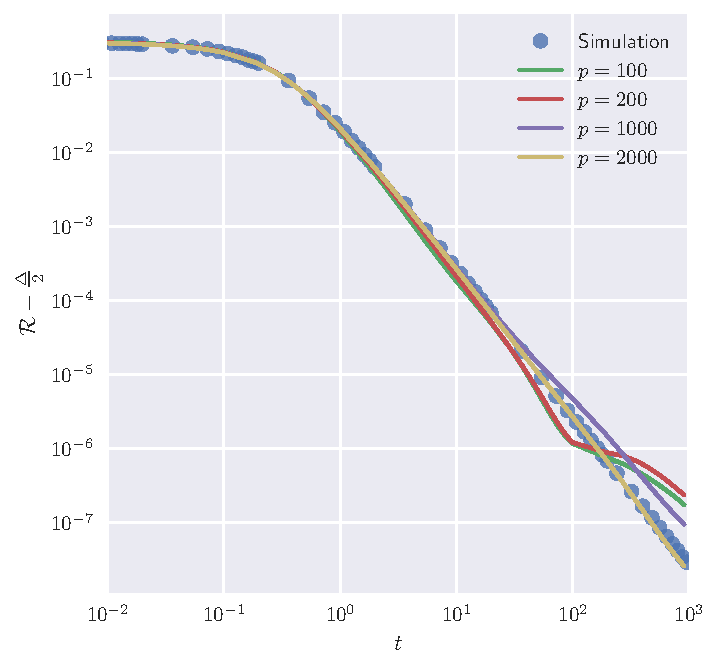
\includegraphics[width=0.49\textwidth]{figs/mean-field/mf_limit_lowdim,offdiag_-k2_d5_activationsquare_gamma1.0000_noise0.0}
        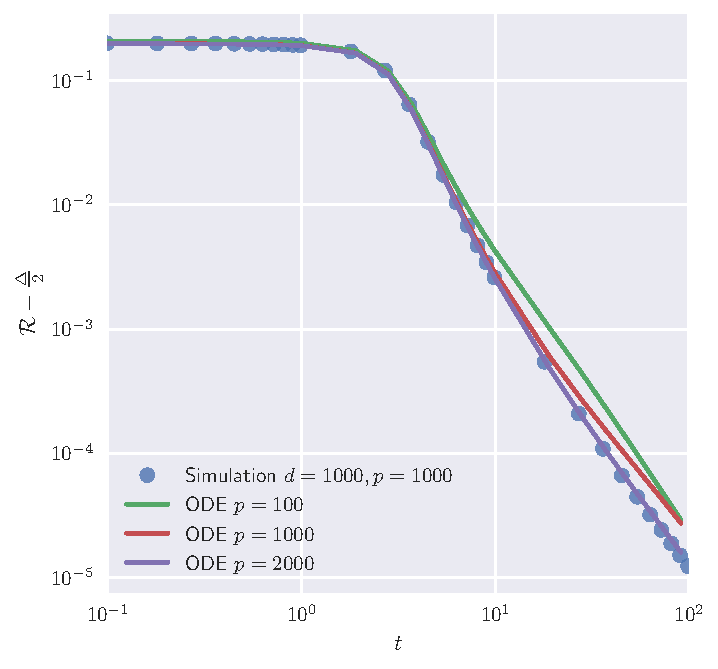
\includegraphics[width=0.49\textwidth]{figs/mean-field/mf_limit_highdim_-k5_activationsquare_gamma10.0000_noise0.0}
    \caption{{\bf The mean-field regime:}    Comparison between population risks of the simulated learning dynamic and the corresponding deterministic evolution, for (left) mean-field low-dimensional regime with squared activation function (\(\hidt=2,d=5,\lr=\num{1.},\noise=\num{0.}\)) and (right) mean-field high-dimensional regime. Apart from finite size effects, there is agreement between ODEs and simulated dynamics (\(\hidt=5,d=1000,\lr=\num{10.}\)).
    }
    \label{2302:fig:meanfield-limit}
\end{figure}
\paragraph{The high-dimensional limit of mean-field:} When $d \to \infty$, the off-diagonal entries of the matrix $\Xi$ are of order $\sfrac{1}{\sqrt{d}}$, which suggests that they can be neglected safely. We therefore define the following equivalent of $\Omega_{\mathrm{MF}}$, which does not depend on auxiliary random variables:
\begin{equation}
    \label{2302:eq:def:overlaps_mf_highdim}
    \bar\Omega = \begin{pmatrix} \bar Q & M \\
        M^\top & P 
    \end{pmatrix}, \quad \bar Q = MP^{-1}M^\top + \mathrm{diag}(q)
\end{equation}
The following lemma then holds:
\begin{lemma}\label{2302:lem:Psi_lipschitz}
    For any $(M, q)\in \mathbb{R}^{p(k+1)}$, we have:
    \begin{equation}
    \left\lVert\mathbb{E}_{\Xi}\left[\Psi^{(M)}(\tilde\Omega)\right] - \Psi^{(M)}(\bar\Omega)\right\rVert_\infty \leq \frac{C}{\sqrt{d}} ,
    \text{and}  
     \left\lVert\mathbb{E}_{\Xi}\left[\Psi^{(\bot)}(\tilde\Omega)\right] - \Psi^{(\bot)}(\bar\Omega)\right\rVert_\infty \leq \frac{C}{\sqrt{d}} .
\end{equation}
\end{lemma}
We thus define the high-dimensional equivalent of \eqref{2302:eq:def:mf_ode}:
\begin{equation}
    \label{2302:eq:def:ode_mf_highdim}
    \frac{\dd{M}}{\dd{t}} = \Psi^{(M)}(\bar \Omega) \qquad \frac{\dd{q}_i}{\dd{t}} = \Psi^{\bot}_{ii}(\bar \Omega).
\end{equation}
The same propagation of perturbations arguments discussed in Appendix B of \cite{veiga2022phase}, and the Lipschitz property of the risk, easily imply the following theorem:
\begin{theorem}
    Under Assumptions \ref{2302:assump:activation} \& \ref{2302:assump:init}, let $\Omega(t)$ and $\bar{\Theta}(t)$ denote the solutions of the ODES \eqref{2302:eq:def:gf_ode} and \eqref{2302:eq:def:ode_mf_highdim}, respectively. Then with probability at least $1 - e^{-z^2}$ on the initialization:
    \[ \sup_{t \in [0, T]} \left| \mathcal R(\Omega(t)) - \mathcal R(\bar{\Theta}(t)) \right| \leq Ce^{CT}\left(\frac{\sqrt{\log(pT)} + z}{\sqrt{p}} + \frac1{\sqrt{d}} \right) \]
\end{theorem}
This approximation eliminates the need to compute expectations in \eqref{2302:eq:def:mf_ode}. We now argue that this phenomenon is not only a consequence of rotation invariance, but also a simple concentration result. Indeed, irrespective of Assumption \ref{2302:assump:init}, we show the following result:
\begin{equation}\label{2302:eq:mf:concentration}
    \left|\mathbb E_{\vec{\lambda^\star}, \vec{\lambda^\bot} \sim \mathcal{N}(\vec{0}, \Omega)}\left[\sigma(\lambda_i)\lambda_i^\bot \mathcal E \right] - \mathbb E_{\vec{\lambda^\star}, \vec{\lambda^\bot} \sim \mathcal{N}(\vec{0}, \bar\Omega)}\left[\sigma(\lambda_i)\lambda_i^\bot \mathcal E \right]\right| \leq c \sqrt{Q^\bot_{ii} \cdot \frac{\lVert Q^\bot \rVert_{\mathrm{op}}}{p}},
\end{equation}
For a random sub-gaussian initialization, classical matrix concentration arguments (see \cite{vershynin2018high}, Theorem 4.4.5) imply
\[ \lVert Q^\bot \rVert_{\mathrm{op}} = O\left(1 + \frac pd \right) \]
and common sense arguments (the presence of an attracting force towards $Q^\bot = 0$) indicates that this quantity stays within the same order of magnitude. On the other hand, by Assumption \ref{2302:assump:boundedness}, the $Q_{ii}$ (and hence the $Q_{ii}^\bot$) remain bounded by an absolute constant during the trajectory. We therefore expect, using standard results from ODE perturbation, that

\begin{equation}
    \lVert \bar\Omega(t) - \tilde\Omega(t) \rVert_\infty \leq e^{Ct}\left(\sqrt{\frac1p}+\sqrt{\frac1d}\right).
\end{equation}
Contrary to the low-dimensional regime and the theorem above, this derivation does not require any rotation invariance of the $\vec{w}_i^\bot$; simply, the averaging properties of $\Psi^{(M)}$ are enough to show direct concentration properties on the dynamics.

It is instructive to look at a concrete example where the phenomenology discussed above becomes explicit. Perhaps the simplest one  is given by the square activation $\sigma(x)=x^2$, for which the expectation in Equation~\eqref{2302:eq:def:Psi} can be explicitly expressed in terms of polynomials of the covariance matrices $(\mat{Q}^{\nu},\mat{M}^{\nu}, \mat{P})$ (see Appendix \ref{2302:sec:app:squared} for the derivation):
\begin{equation}
\label{2302:eq:squared_ODE}
\begin{split}
    \Psi^{(\mathrm{M})}(\Omega)   &= 2\left(\frac{\Tr{\P}}k - \frac{\Tr{\Q}}p\right)\M +
        4\left(\frac{\M\P}{k} - \frac{\Q\M}{p}\right) \\
    \Psi^{(\mathrm{GF})}(\Omega)  &= 4\left(\frac{\Tr{\P}}k - \frac{\Tr{\Q}}p\right)\Q +
        8\left(\frac{\M\M^\top}{k} - \frac{\Q^2}{p}\right) \\
    \Psi^{(\mathrm{\bot})}(\Omega) &= 4\left(\frac{\Tr{\P}}k-\frac{\Tr{\Q}}{p}\right) \Q^\bot - \frac{4}{p}\left(\Q\Q^\bot+\Q^\bot\Q\right).
\end{split}
\end{equation}
Similarly, the population risk as a function of the sufficient statistics reads:
\begin{equation} \label{2302:eq:risk_quadratic}\begin{split}
  \mathcal{R}(\Omega)
       =  \frac{\Tr{\P}^2+2\Tr{\P^2}}{2k^2}
           - \frac{\Tr{\P}\Tr{\Q}+2\Tr{\M\M^\top}}{pk}
           + \frac{\Tr{\Q}^2+2\Tr{\Q^2}}{2p^2}
           + \frac\Delta2.
\end{split}\end{equation}

The high-dimensional mean field limit is then particularly simple. Recalling the definition of \(\bar\Omega\) in Equation~\eqref{2302:eq:def:overlaps_mf_highdim}, we obtain  the explicit equations by replacing \(\Omega\) with \(\bar\Omega\). The situation is, however, different for the low-dimensional mean-field limit, due to the randomness introduced by matrix \(\Xi\). The 
ODEs and the risk, given the parameters $\tilde\Theta$, are
\begin{equation}\label{2302:eq:def:mf_square}\begin{split}
    \mathbb{E}_{\Xi}\left[\Psi^{(M)}(\tilde\Omega)\right] &= \Psi^{(M)}(\bar\Omega) \qquad
    \mathbb{E}_{\Xi}\left[\Psi^{(\mathrm{noise})}(\tilde\Omega)\right] = \Psi^{(\mathrm{noise})}(\bar\Omega) \\
    \mathbb{E}_{\Xi}\left[\Psi^{\bot}_{ii}(\tilde\Omega)\right] &= \Psi^{\bot}_{ii}(\bar\Omega) - \frac8p \frac{\sum_{j=1,j\neq i}^\hids q_j}{d-k}q_i \\
    \mathbb{E}_{\Xi}\left[\mathcal{R}(\tilde\Omega)\right] &= \mathcal{R}(\bar\Omega) + \frac{1}{p^2} \frac{\sum_{i=1}^\hids\sum_{j=1,j\neq i}^\hids q_iq_j}{d-k}.
\end{split}\end{equation}
In this case, the low-dimensional corrections are therefore just additive terms. As expected, these corrections vanish when \(d\to\infty\), where we fall back to the high-dimensional mean-field. Conversely, when \(d= k\) the correction diverges, but we don't need to track \(q\) anymore since the teacher weights are spanning the whole space \(\mathbb{R}^d\), and the orthogonal space is null; hence \(\Q^\bot = 0\) and this is a stable point of the dynamics. In Figure~\ref{2302:fig:meanfield-limit} we show some numerical experiments using this activation function; for a more detailed discussion see Appendix~\ref{2302:sec:app:numerics-mean-field}.
% %%%%%%%%%%%%%%%%%%%%%%%%%%%%%%%%%%%%%%%%%%%%%%%%%%%%%%%%%%%%%%%%%%%%%%%%%%%%%%%
